%
\documentclass[longbibliography,nofootinbib]{revtex4-1}
\usepackage{xeCJK}
\newcommand{\kms}{NuCypher KMS}

\usepackage{listings}
\usepackage{graphicx}
\usepackage{amsmath}
\usepackage[margin=5pt]{subfig}
\usepackage[usenames]{color}


\renewcommand{\baselinestretch}{1.4}
\setlength{\parskip}{1em}
\setlength{\parindent}{20pt}
\definecolor{darkgreen}{rgb}{0.00,0.50,0.25}
\definecolor{darkblue}{rgb}{0.00,0.00,0.67}
\usepackage[breaklinks,pdftitle={NuCypher KMS: decentralized key management system (Chinese translation)}, pdfauthor={Michael Egorov},colorlinks,urlcolor=blue,citecolor=darkgreen,linkcolor=darkblue]{hyperref}
\graphicspath{{pdf/}}
\def\andname{和}

\begin{document}

\renewcommand{\tocname}{内容}
\renewcommand{\figurename}{图}
\newcommand{\figref}[1]{图\ref{#1}}

\title{\kms : 去中心化密钥管理系统}

\author{Michael Egorov}
\email{michael@nucypher.com}
\author{MacLane Wilkison}
\email{maclane@nucypher.com}
\affiliation{NuCypher}

\author{David Nu{\~n}ez}
\email{dnunez@lcc.uma.es}
\affiliation{NICS 实验室, 马拉加大学, 西班牙}
\date{一月四号, 2018}

\author{翻译:Zhen Zou, Z, tobeaj2mer01}

\begin{abstract}
    \kms 是一个去中心化密钥管理系统(KMS),它解决了使用共识网络安全存储和操作私有加密数据的问题\cite{cryptoeprint:2017:201}。
    它利用代理重加密技术,使用去中心化网络,提供基于加密和密码学的权限控制\cite{wiki:pre}。
    不像中心化的KMS提供的服务,它不需要信任服务提供商。
    \kms 使共享敏感数据给去中心化和中心化的应用程序成为可能,为从医疗到ID管理再到去中心化内容市场的众多应用程序提供安全架构。
    \kms 会成为去中心化应用程序必要的一部分,就像SSL/TLS是每个安全的网络应用程序必要的一部分一样。
\end{abstract}

\maketitle

\tableofcontents

\newpage

\section{摘要}

\kms 是一个去中心化密钥管理系统(KMS),提供加密和权限控制服务。
它能够在共识网络上在任意数量的参与者之间共享私有数据,使用代理重加密技术来管理解密权限,这是传统对称加密和公钥加密方案不能实现的。
代币用来激励网络参与者执行密钥管理和权限的授权/撤销操作。

\subsection{背景}
权限管理系统(KMS)是在设备和应用程序中生成、分发和管理密钥的集成方案(\figref{fig:kms})。
KMS包含在设备上生成、分发和流转密钥的后台功能以及注入、存储和管理密钥的客户端功能\cite{wiki:kms}。

\begin{figure}
    \centering
    \subfloat[中心化KMS]{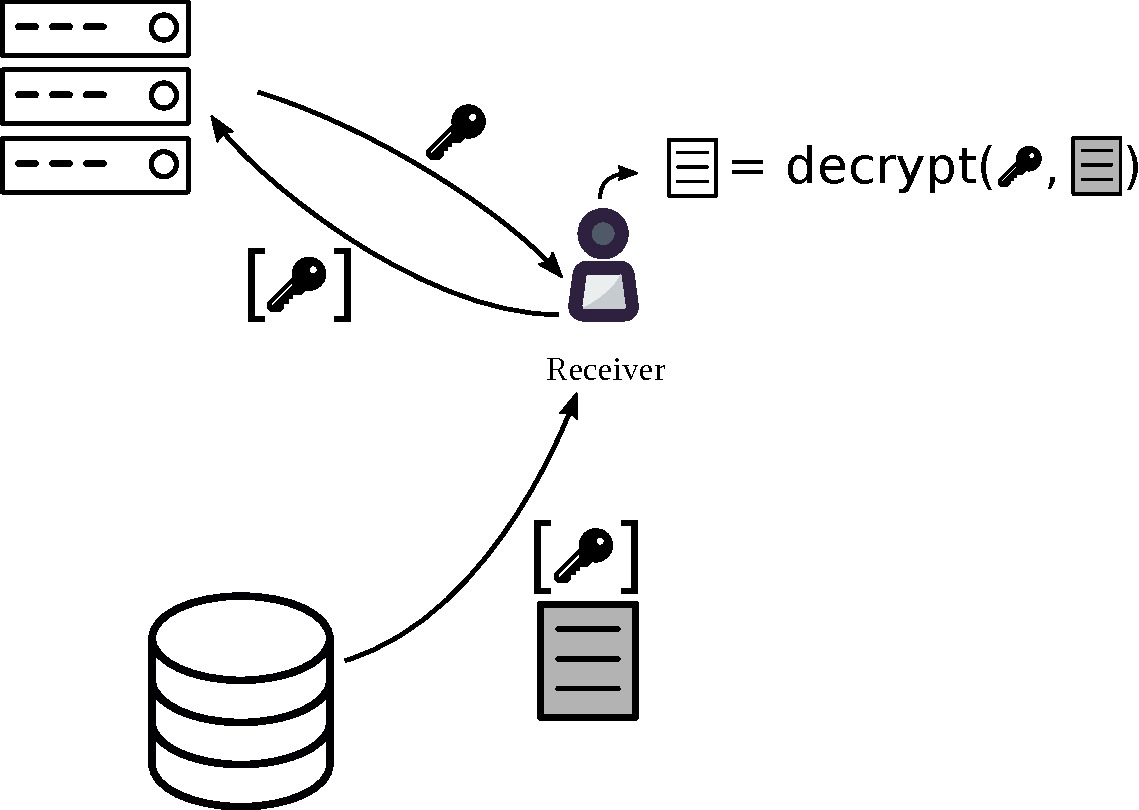
\includegraphics[width=0.4\columnwidth]{pdf/centralized-kms.pdf}}
    \qquad
    \qquad
    \subfloat[代理重加密KMS]{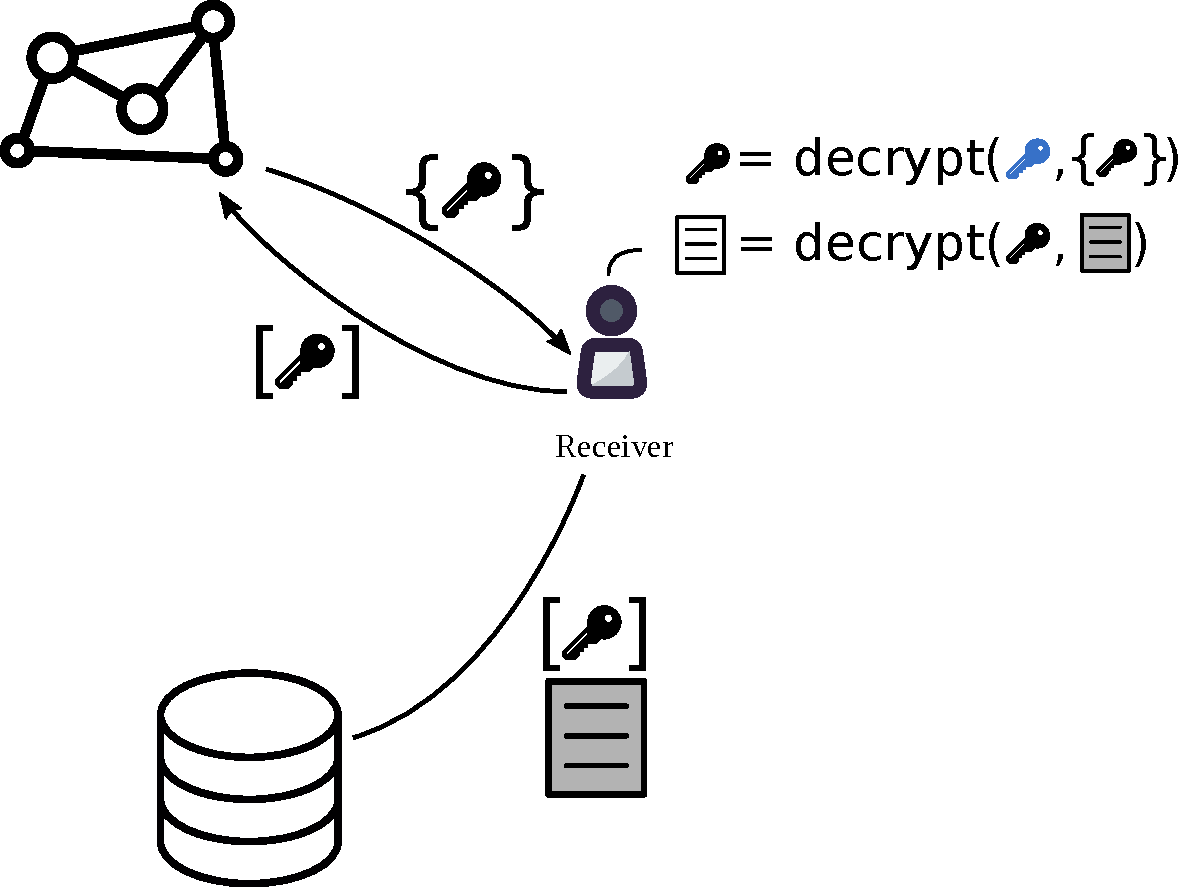
\includegraphics[width=0.4\columnwidth]{pdf/pre-kms.pdf}}
    \caption{中心化密钥管理系统(KMS)和代理重加密(PRE)密钥管理系统的区别}
    \label{fig:kms}
\end{figure}

作为信任的根源,适当配置、管理和保护KMS很关键。
传统上,这意味着把KMS部署到硬件安全模块(HSM)\cite{wiki:hsm} 或者使用诸如HashiCorp's Vault\cite{web:hashicorp-vault}这样的工具。
然而这需要很高等级的技术复杂性和前期资本投入,为了降低技术负担和提供有竞争力的价格,像亚马逊云HSM\cite{web:aws-cloudhsm},
谷歌云KMS\cite{web:google-cloud-kms},微软Azure Key Vault\cite{web:azure-key-vault}和TrueVault\cite{web:truevault} 等供应商开始提供KMS服务。
然而,KMS作为服务产品需要在服务提供商中设置不适当的信任级别,这对于强调安全的应用程序而言可能并不合适。

诸如比特币和以太坊这样的共识网络在解决这种中心化的难题方面很有前途。但是,在公众共识网络上执行涉及私密数据操作的局限性是已被确认的\cite{cryptoeprint:2017:201}。
共识网络采用一个志愿者节点网络,在可用性和强制访问管理规则方面,这种网络经常发生中断,而不像中央基础设施那样可靠。

\kms 使用去中心化网络移除对中心化服务提供商的依赖,使用代理重加密提供密码访问控制,使用代币激励机制保证可靠性、可用性和正确性。
由于使用代理重加密,未加密的对称密钥(能够解密私有数据)绝不会暴露在服务器端(\figref{fig:kms}),并且不会出现单点安全失败。
即使被攻破,黑客也只能得到重加密的密钥,而对文件的访问仍然受到保护。

\section{架构}

\subsection{加密基元}

\subsubsection{对称加密}

对称或私钥加密要求用户知道一个公共秘密密钥。
为了方便起见,我们将这个公共密钥称为DEK(数据加密密钥)。

对称加密定义了两个操作:
\begin{align}
    c &= \text{encrypt}_{sym}(dek, d);\\
    d &= \text{decrypt}_{sym}(dek, c);
\end{align}
$d$是明文,$c$是密文(加密数据)。

对于我们来说,最有用的对称密钥加密算法是AES(因为它通常是硬件加速的)\cite{wiki:aes}和Salsa20 \cite{wiki:salsa20}。

对称分组密码可以在不同的模式下运行。
我们使用概率加密的操作模式(如用于AES的GCM)来保证强大的语义安全性。
为了简单起见,我们省略了关于特定操作模式的细节,将与操作模式有关的随机数值视为密文的一部分$c$。

\subsubsection{公钥加密}

公钥加密(PKE)是双方(发送方和接收方)无需公钥即可交换信息的一种加密方式。
每个参与者都有一个密钥对(一个公钥$pk$和一个密钥/私钥$sk$)。
如果发送方有一个密钥对$sk_s/pk_s$,并且接收方有一个密钥对$sk_r/pk_r$,发送方可以使用接收方的公钥对消息进行加密,接收方可以用他的密钥进行解密。

可以创建混合密码系统,将对称加密的效率与PKE的便利性结合起来。
混合密码系统加密流程定义了以下函数:
\begin{align}
    dek &= \text{random}();\\
    c &= \text{encrypt}_{sym}(dek, d);\\
    edek &= \text{encrypt}_{pke}(dek, pk_r).
\end{align}
该对$(edek,c)$用于转换加密的数据。
接收方的相关解密定义了以下函数:
\begin{align}
    dek &= \text{decrypt}_{pke}(edek, sk_r);\\
    d &= \text{decrypt}_{sym}(dek, c).
\end{align}

\subsubsection{代理重加密}
代理重加密(PRE)\cite{wiki:pre,nunez2017proxy}是一种公钥加密(PKE),它允许代理实体将密文从一个公钥转换到另一个公钥,而不需要知道任何关于底层消息的信息(\figref{fig:pre})。

\begin{figure}
\centering
    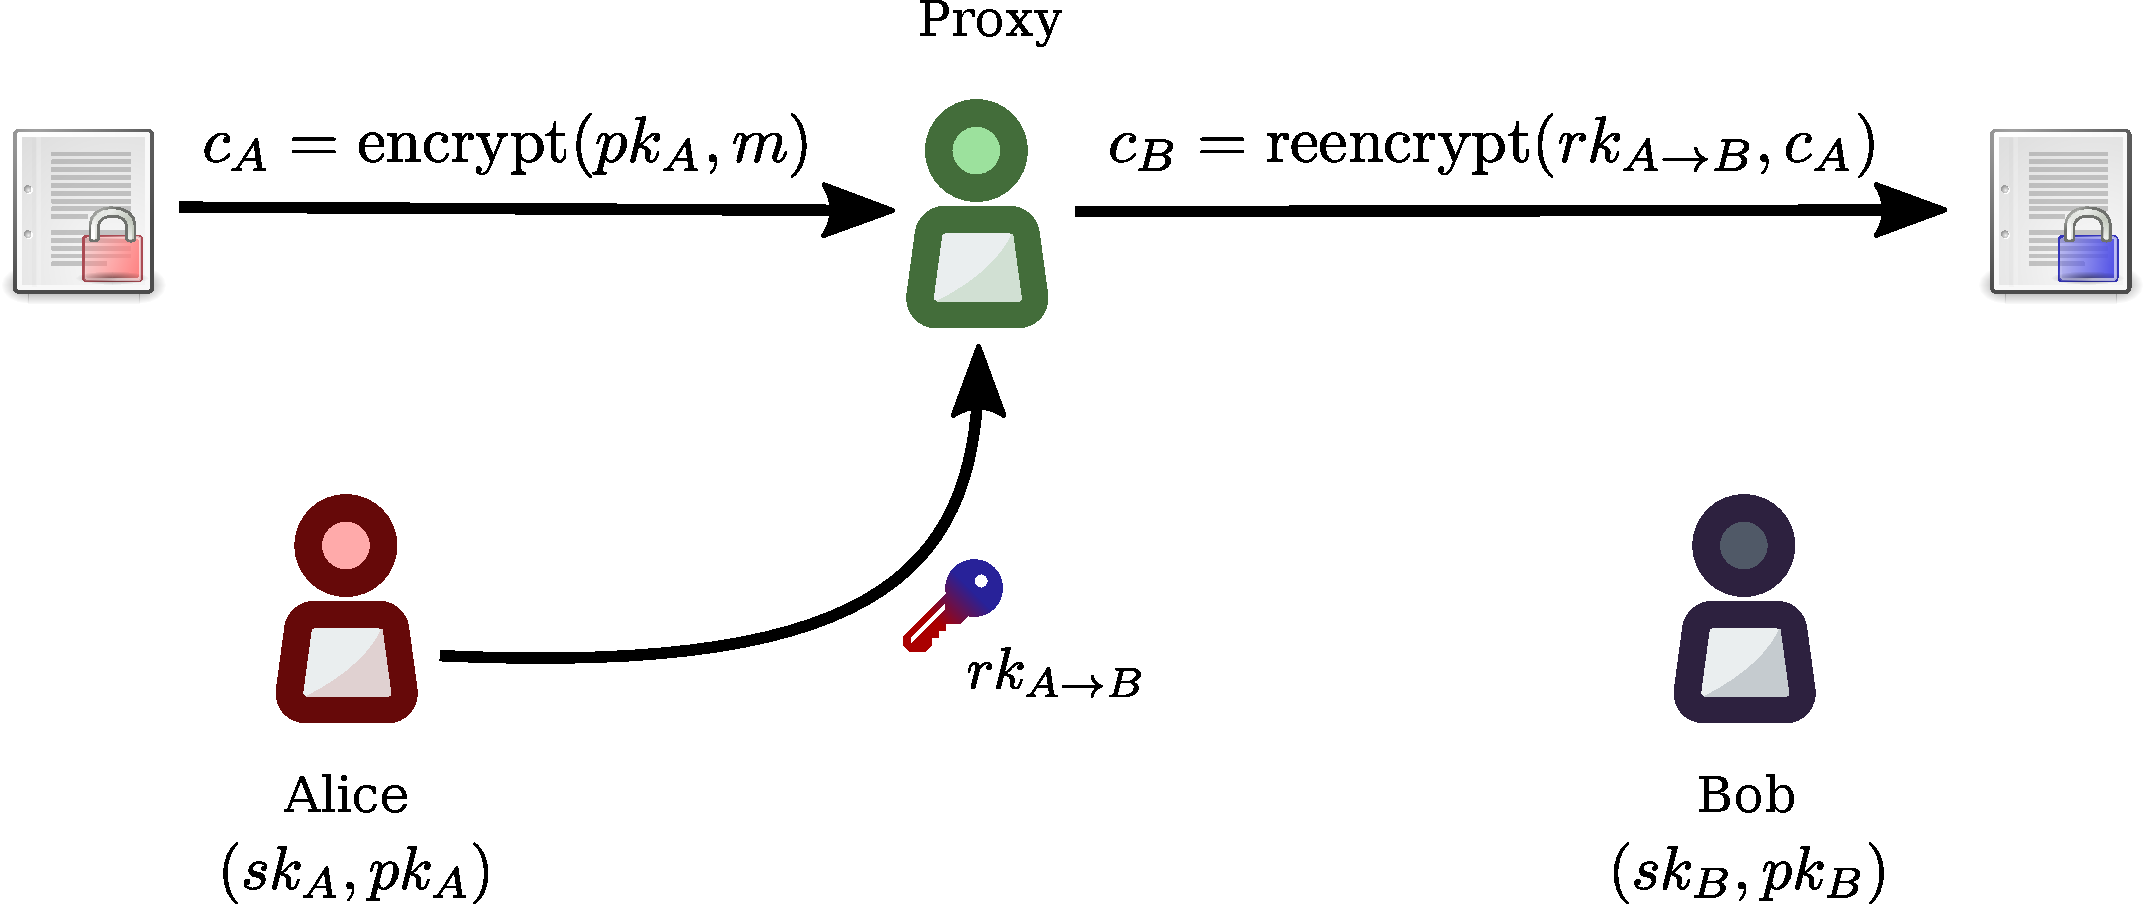
\includegraphics[width=0.6\columnwidth]{pdf/pre.pdf}
    \caption{代理重加密环境中的主要参与者和交互}
    \label{fig:pre}
\end{figure}

在典型的代理重加密的情况下有几个角色,
数据拥有者Alice拥有公钥$pk_A$。
知道这个密钥的任何实体都可以使用她的密钥$sk_A$产生只有她可以解密的加密数据。
假设数据生产者用Alice的公钥$pk_A$加密消息$m$,得到密文$c_A$.
Alice决定把对m消息的访问权委托给拥有密钥对$(pk_B, sk_B)$的Bob。
为此,Alice创建一个重密密钥:
\begin{equation}
    rk_{A\rightarrow B} = \text{rekey}(sk_A, pk_B).
\end{equation}
重要的是,在单次使用的单向代理重加密方案中,这种重加密函数是一种方式,并且$rk_{A\rightarrow B}$不能被分解成其组成部分(至少在不知道$sk_A$或$sk_B$的情况下)。
它所能做的就是对$c_A$进行重加密,以便将其转换为$c_B$:
\begin{equation}
    c_B = \text{reencrypt}(rk_{A\rightarrow B}, c_{A}).
\end{equation}
Bob然后可以用他的秘密密钥$sk_B$解密$c_B$。

与现有的适合1对1通信的PKE协议相较,代理重加密在任意数量的数据生产者和消费者的N对N通信时更具可扩展性。
它不需要事先知道消息的接收方,因为重加密令牌可以在任何时候被创建和使用。
这使得它非常适合去中心化系统,如区块链、物联网和大数据~\cite{web:nucypher-hadoop}。

有许多具有不同属性的代理重加密算法。
对于\kms 的第一个版本,我们选择了ECIES,我们为其创建了代理重加密算法\cite{umbral-spec}。
它与最简单的(和高性能的)算法BBS98~\cite{BBS98}非常相似,但提供了更好的安全保证。
然而,有时我们想要将重加密委托给多个节点,以便拆分它们之间的依赖并应用基于时间的或有条件的重加密策略。
在这种情况下,我们使用AFGH方案\cite{AFGH}。
抗量子的NTRU在有需要时也可使用\cite{wiki:ntru,ntrureencrypt}。

就像BBS98一样,我们对ECIES的代理重加密算法是利用两个私钥创建一个重加密密钥,而不是一个私钥+公钥。
但是,我们不希望发送方知道接收方的密钥。
为了解决这个问题,我们随机生成一个临时密钥对$sk_e/pk_e$。
然后,访问委托看起来像这样:
\begin{align}
    \label{eq:ephemeral-trick}
    sk_e &= \text{random}();\\
    rk_{A\rightarrow e} &= \text{rekey}(sk_A, sk_e);\\
    \label{eq:ephemeral-trick-end}
    sk_e^{\prime} &= \text{encrypt}_{pke}(pk_B, sk_e);\\
    rk_{A\rightarrow B} &= (rk_{A\rightarrow e}, sk_e^{\prime});
\end{align}

重加密节点使用$rk_{A\rightarrow e}$重加密任何密文$c_A$(其基础消息为$m$),以便可以通过$sk_e$解密。
由于接收方需要使用$sk_e^{\prime}$对重加密的密文进行解密,因此将其附加到重加密的结果上。
因此,重加密的过程如下:
\begin{align}
    c_e = \text{reencrypt}(rk_{A\rightarrow e}, c_{A});\\
    c_B = (c_e, sk_e^{\prime});\\
\end{align}

接收方的解密将如下所示:
\begin{align}
    sk_e &= \text{decrypt}_{pke}(sk_B, sk_e^{\prime});\\
    m &= \text{decrypt}_{pke}(sk_e, c_e);\\
%    d &= \text{decrypt}_{sym}(dek, c).
\end{align}

Ateniese等人\cite{AFGH}事先提到了这种方法,这也超出了代理重加密的范围。
该方案不被认为是“密钥优化”的,但在我们的用例中,却却拥有非常有竞争力的性能。

\subsection{重加密方案的简要回顾}

重加密方案有不同的属性。在本小节中,我们考虑其中几个与我们用例有关的属性。 一个关于所有已知的代理重加密算法及其属性的全面调查已于近期发布~\cite{nunez2017proxy}.

要考虑的重要属性之一是算法是否是交互式的。 “交互式式”意味着重加密密钥是由两个密钥计算出来的:
\begin{equation}
    re_{ab} = \text{rekey}(sk_a, sk_b).
\end{equation}
“非交互”意味着需要知道所有者的私钥和被授权者的公钥:
\begin{equation}
    re_{ab} = \text{rekey}(sk_a, pk_b).
\end{equation}

交互算法的例子有:BBS98~\cite{BBS98},我们的ECIES重加密算法(基于BBS98)和基于LWE的重加密算法~\cite{lwe-reencryption}。一个“非交互式”算法的例子是AFGH~\cite{AFGH}。 尽管最初似乎我们只对非交互式算法感兴趣,但我们可以通过使用临时密钥(方程~\ref{eq:ephemeral-trick}-\ref{eq:ephemeral-trick-end})在协议级别调整非交互式算法,以便与公钥而不是私钥共享。

另一个有趣的属性是算法是单向的还是双向的。双向性意味着可以从$re_{ab}$计算$re_{ba}$,这在单向算法中是不可能的。但是当使用临时密钥时,双向算法实际上就是单向算法(方程~\ref{eq:ephemeral-trick}-\ref{eq:ephemeral-trick-end})。尽管如此,我们在Sec.VC中展示单向性可以非常方便地以可扩展的方式共享复杂的分层数据。一个双向算法的例子是BBS98~\cite{BBS98}。

    代理重加密算法也可以是单跳或多跳的。 “多跳”是指如果我们有了$re_{ab}$和$re_{bc}$,那么这两个重加密的密钥可以串联使用,在不需要$b$的情况下将密文$c_a$转换成密文$c_c$ :

\begin{equation}
    c_c = \text{reencrypt}(re_{bc}, \text{reencrypt}(re_{ab}, c_a)).
\end{equation}
有时甚至可以计算$re_{ac}$,对于BBS98是这样的::
\begin{equation}
    re_{ac} = re_{ab} \cdot re_{bc}.
\end{equation}

“单跳”是指如果通过重加密获得$c_b$,则不可能进一步对其进行重加密。多跳方案对于密钥轮换(Sec.~\ref{sec:key-rotation})和我们的分层数据共享方案(Sec.~\ref{sec:hierarchical-data})是有用的。临时密钥(方程~\ref{eq:ephemeral-trick}-\ref{eq:ephemeral-trick-end})是临时单跳(只有当数据与其他方共享时才会创建临时密钥,因此密钥轮换是可能的)。 多跳算法的例子包括BBS98~\cite{BBS98} 和基于LWE的算法~\cite{lwe-reencryption}。 AFGH算法~\cite{AFGH}是单跳的。

另一个看似重要的属性是抗合谋。非正式地说,抗合谋意味着只获得$re_ab$和$sk_b$是不可能派生出$sk_a$的。相反,缺乏抗合谋使得可以从$re_{ab}$和$sk_b$获得$sk_a$。 乍一看,这似乎是非常安全的。 然而,即使使用抗合谋算法,如果攻击者同时拥有reab和skb,他也能够重加密和读取任何原本只能由$sk_a$解密的数据。因此,只有当相同的密钥对用于其他目的(例如签名,密钥导出等)时,抗合谋性才变得很重要。尽管如此,为两个函数使用单独的密钥对是一种好的做法。 就我们的目的而言,抗合谋似乎并不是一个优先事项,因为除了加密之外,我们没有另外使用委托人的密钥对的地方。 抗合谋算法包括AFGH~\cite{AFGH} 和基于LWE的重加密算法~\cite{lwe-reencryption}。 非抗合谋算法是BBS98~\cite{BBS98}和ECIES。


我们可能需要使得重加密密钥中的数据的生产者和/或消费者无法被识别(第~\ref{sec:anonymity}节)。 通常,知道系统中所有公钥的代理能够推断出这些信息。 从重加密的角度来看,许多PRE方案并不是匿名的~\cite{BBS98,AFGH}。 然而,基于LWE的重加密方案 ~\cite{lwe-reencryption}享有匿名性。

最后,对于任何密码系统,CPA安全性~\cite{wiki:cpa}(选择明文攻击安全性)和CCA安全性~\cite{wiki:cca}(针对选择密文攻击的安全性)的概念适用于代理重加密。 除了也具有CCA安全的ECIES和LWE重加密以外,到目前为止我们提到的所有算法都只是CPA安全的~\cite{lwe-reencryption}。

% XXX check

\subsection{签署加密消息}

    在公钥加密算法中,任何人都可以使用$pub_a$进行加密。 虽然这很有用,但是它也允许网络的恶意用户加密数据,就好像它们是$A$.因此,数据必须被签名以便向接收方证明发送方的身份。
    
    但是,我们希望使协议匿名化(第IIIA节)成为可能,因为验证数据所有者的公共数字签名也提高了重加密节点尝试向所有者索取钱财的可能性。因此,这样做是合理的:

\begin{itemize}
    \item 将数字签名作为明文的一部分,这样在密文解密之前不可能验证签名
    \item 使用不同的密钥对进行签名和加密(特别是考虑到某些重加密密码系统缺乏抗合谋性)
\end{itemize}

\subsection{重加密节点}

当数据存储在云或去中心化存储系统中时,其是被数据所有者(发送方)的密钥$pk_s$(\figref{fig:arch-encrypt}) 所加密的。数据本身被随机对称密钥$dek$加密,每个文件一个密钥。 用$pk_s$加密的$dek$被附加到加密的数据上。 这个组合 $(edek,c)$ 可以存储在任何地方 - IPFS,Swarm,S3或者任何类型的去中心化或中心化存储系统中。

\begin{figure}
\centering
    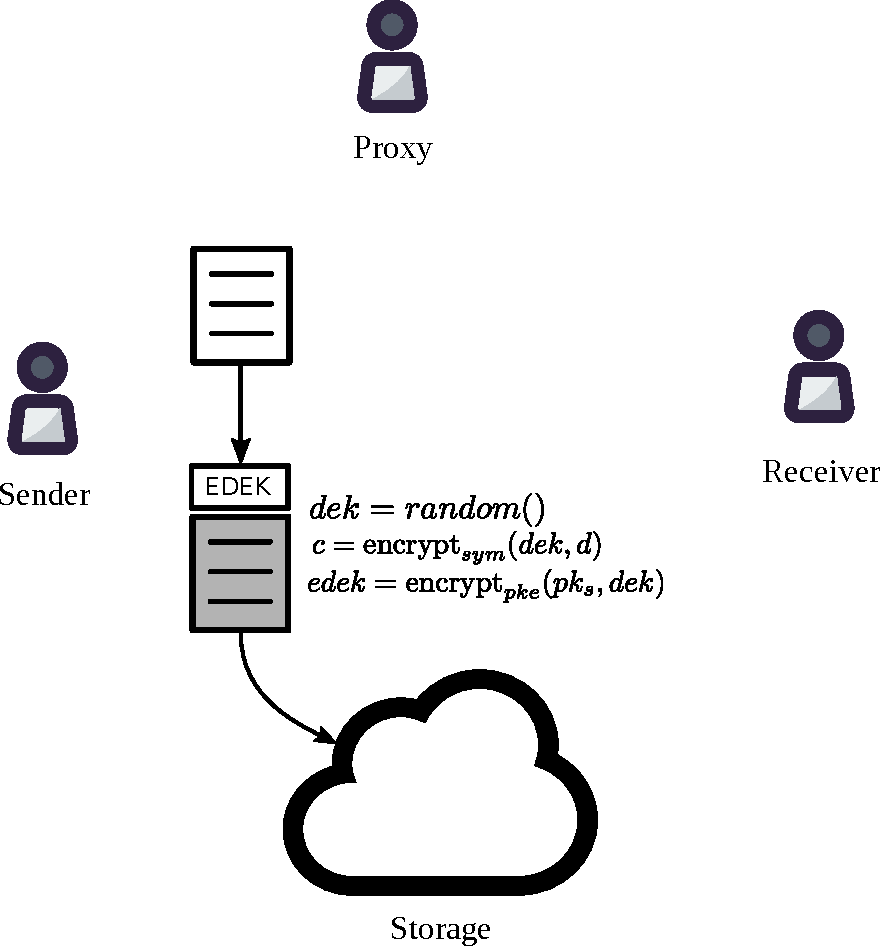
\includegraphics[width=0.4\columnwidth]{pdf/encrypt.pdf}
    \caption{架构:加密}
    \label{fig:arch-encrypt}
\end{figure}

在存储数据时,我们委托访问的用户不一定是事先知道的。 首先,接收方应该向发送方显示他的公钥 ~(\figref{fig:arch-delegate})。 公钥对应于以太坊网络中的地址通常是有意义的(例如,证明已经从用于数字内容订阅的该地址进行了支付)。 发送方生成一个重加密密钥(在需要的时候包括一个加密的随机临时密钥),并将其发送到一个随机重加密节点,根据PoS在去中心化网络中选择活动结点。 稍后将讨论为了冗余或安全而选择多个节点的情况。在发送方用户和接收方用户间分享数据的节点将该信息登记在网络中。

当接收方想要解密与他共享的数据时,他首先从数据存储器或加密数据流中下载该数据~(\figref{fig:arch-decrypt})。 他将$edek$从消息中分离出来并将$edek$发送到重加密节点的网络,并找到可以与接收方(具有重加密密钥的那些)共享发送方的数据的活动重加密节点。接收方请求具有重加密密钥的节点将$edek$转换为$edek^{\prime}$并使用他自己的密钥skr对其进行解密并获得$DEK$。 现在,他可以使用DEK来解密大量的数据。

\begin{figure}
\centering
    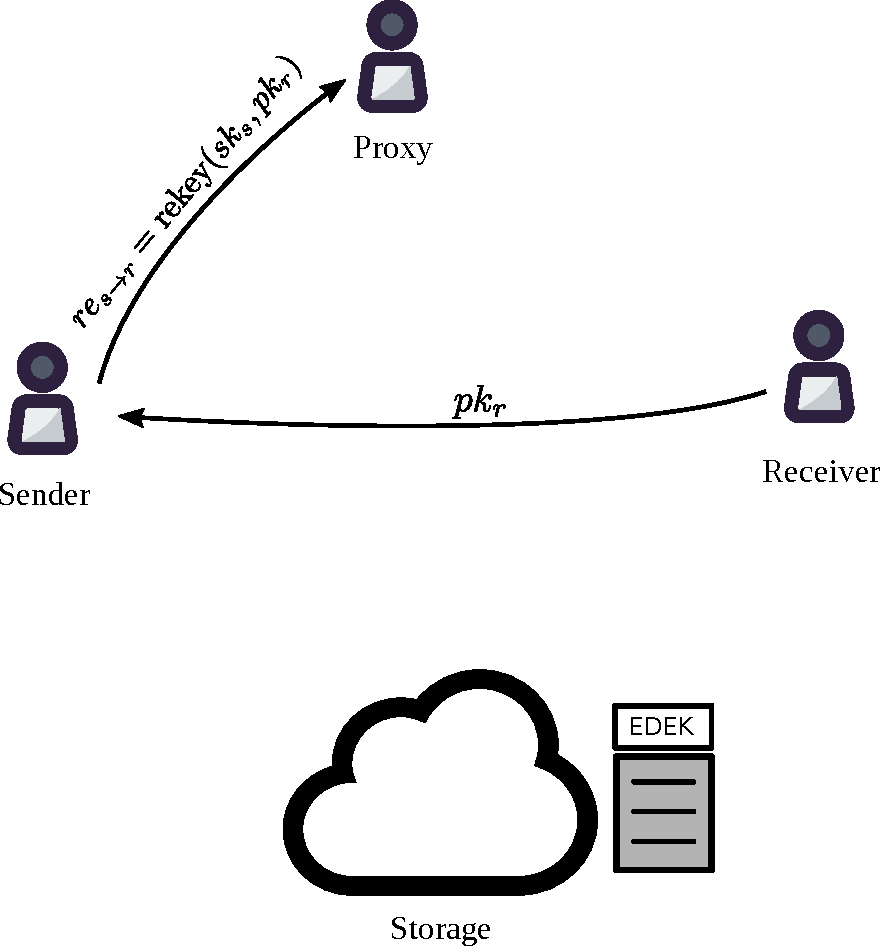
\includegraphics[width=0.4\columnwidth]{pdf/delegate.pdf}
    \caption{架构:访问委托}
    \label{fig:arch-delegate}
\end{figure}

\begin{figure}
\centering
    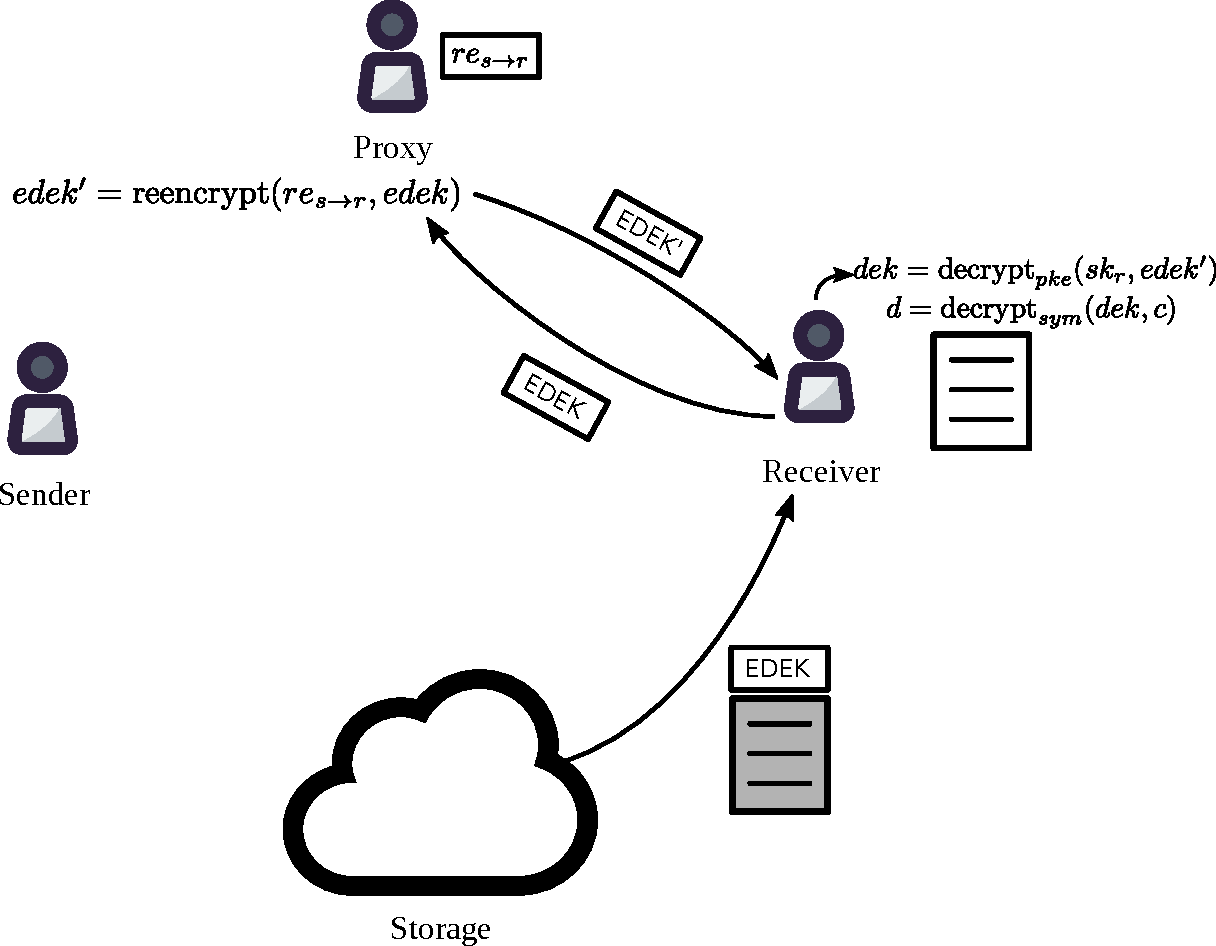
\includegraphics[width=0.6\columnwidth]{pdf/decrypt.pdf}
    \caption{架构:解密}
    \label{fig:arch-decrypt}
\end{figure}

\section{网络安全}

在网络中,有多个应用访问管理策略的重加密节点。

    代理重加密允许NuCypher KMS在访问管理和解密权限之间拆分依赖,而无需引入始终在线且一直可信的实体(如传统的密钥管理系统)。 矿工始终不能看到明文数据,或者任何能够解密数据的东西。 他们只是负责存储重加密密钥并应用重加密函数。
    
    这种模式的第一个风险是矿工和数据读取器之间的共谋。 如果矿工给数据读取器提供数据的重加密密钥,数据可以在任何时候由数据读取器解密,这将使任何有条件的或基于时间的约束失灵。我们以多种方式抵制这种威胁,包括重加密密钥的伪匿名、分割密钥代理重加密和挑战协议。另外,我们运用经济激励措施以保障公平运行,这在第~\ref{sec:token}章中有详细描述。

第二个风险是节点发生故障(返回错误数据而不是执行重加密)。 我们使用挑战协议解决这个问题。

第三个风险是节点相互共谋,进行50%攻击。这通常对多方参与的计算是致命~\cite{vitalik-secret-dao}(如Enigma~\cite{enigma})。 但是,对我们而言,攻击者只能获得错误应用重加密策略的能力,而不能解密数据或向其他未被授权的用户提供授权。 理想情况下,系统应尽可能去中心化,然而50%攻击不会危及数据的机密性,就像在应用工作量证明机制的加密货币中,50%攻击不会给攻击者移动资金的能力。

\subsection{伪匿名}
\label{sec:anonymity}

重加密节点不知道他们正在重加密的是什么对于系统的安全性是非常有益的。 这样可以防止他们知道重加密密钥以应对共谋攻击(并且在去中心化网络中试图与所有网络参与者共谋是不可行的)。 而且,重加密密钥的伪匿名也使我们能够运行挑战协议(章节.~\ref{sec:challenge-protocol})

我们把设计一个匿名重加密协议作为未来的改进。 但是,我们指出它应该(不应该)拥有下列属性。首先,重加密方案应该是密钥私有的~\cite{Ateniese-key-private,lwe-reencryption}。否则,可以通过遍历所有已知的公钥对来确定密钥的所有权。 其次,重加密节点和数据的接收方对于相同的重加密密钥不应该具有相同的标识符。 这就排除了将重加密密钥存储在密钥-值对存储中的简单做法,而接收方可以拿出密钥。

\subsection{分割密钥重加密}
\label{sec:split-key}

有一种情况,重加密的节点决定立即重新加密数据而不是根据设置好的条件策略加密数据。 分割密钥代理重加密方案可以用来解决这个问题。
    相对于一个重加密密钥,m-m重加密密钥可以用来产生“重加密共享”。这些共享可以在客户端结合。AFGH~\cite{AFGH}加密使用m-m方案,这里的共谋攻击将需要$m$个矿工和数据读取器。
    
    我们与马拉加大学的NICS实验室共同开发的基于阈值的m-n方案(Umbral)似乎更适合于这项任务。 该方案还可以允许第三方验证重加密的正确性,这对于保持节点的诚实是重要的。

\subsection{挑战协议}
\label{sec:challenge-protocol}

矿工返回随机数字而不是正确地重加密数据是一种风险。 由于数据是私密的,所以系统的用户不能公布这些数据和他们的密钥来证明矿工已经作弊。

    矿工不可能区分“真正的重加密”和随机数据的重加密。 所以,我们可以生产一些专门为挑战矿工而设计的“假”重加密密钥。 如果矿工作弊,这个用于挑战的数据和密钥不与任何私有数据相关联。
    
    矿工应当把数据重加密之前和之后的哈希值展示到网络之中。 如果这种重加密数据是挑战协议数据,而且矿工已经作弊,那么挑战者可以展示一个证据,证明与这个挑战相关的非敏感密钥实际上应该产生不同的重加密结果,同时矿工的抵押资产可以奖励给挑战者。
    
    正如Truebit~\cite{truebit}所指出的那样,系统还应该有意地产生一些“错误的重加密数据”,以激励挑战者进行挑战。

        设计一个挑战协议是一个与“公平交换”协议有关的复杂问题~\cite{BitcoinMPC2016,Bentov2014,AccountableStorage}。 这需要仔细的设计和测试,而以太坊的权益证明(Casper)协议现在也面临着这样的复杂性。只在加密算法层面上检验正确性是可行的~\cite{Zhou2002}。
    
    应该特别考虑保护重加密密钥免于泄漏。建议以下挑战协议。
    
    当承担重加密密钥的责任时,矿工希望随着时间$T$获得费用$f$,因此数据的所有者需要存储$f$个币。 矿工还应该提供抵押品$c$,如果重加密密钥泄露,将被没收。

        如果一个挑战者证明矿工已经泄漏了一个重加密密钥,挑战者应该得到奖励。 然而,数据所有者可能会挑战矿工,以欺诈方式获得挑战奖励。我们使这个“自我挑战”变得不可行。 如果挑战发生在时间$t$之后,挑战者将获得 $\alpha f t/T$ 硬币,其中$\alpha < 1$。在这种情况下,数据拥有者获得  $(1 - t/T) f$  个币。抵押品和剩余费用被分给网络的其他参与者,总金额为 $c + (1 - \alpha) t/T$。

    数据的拥有者挑战矿工时不应该被激励,而是应该使用撤销策略。 因此,在一个“正确的”撤销中,数据的所有者获得$(1 - t/T) f$个币,矿工得到 $c + ft/T$个币,其中$c$是被押的抵押品。
\subsection{不同使用案例中潜在威胁的相关性}

% Mobile Device Management

    在移动设备管理使用案例(第~\ref{sec:mdm}节)中,最重要的是在数据泄露之前从丢失或被盗的设备中撤销权限。想象一下,有人可能会偷窃设备,并与相关矿工共谋。因此,矿工必须不能识别用户,反之亦然。另一个可能的攻击是一组矿工撤销权限并要求为重加密额外支付费用。但是,由于数据所有者可以轻松地重新授予访问该移动设备的权利,所以没有这样做的动机。另一个可能的威胁是挖矿节点在策略生命周期终止后长期留存重加密密钥,等待其他人攻击最终用户的设备并与挖矿节点共谋。 为了防止这种威胁,挖矿节点不能确定数据是否有价值是很重要的,一个好的方法是匿名化数据所有者和数据本身。 换句话说,我们阻止挖矿节点发现$edek$对应的数据。
    
    去中心化DRM(Sec.~\ref{sec:drm})假定一旦内容(一个文件或一段视频)被解密,就已经被购买,所以权限撤销不是真正的问题。但是,如果一个节点知道内容非常昂贵,他们可能试图接近买方,并就内容提出更便宜的价格,从而切断原卖方。 为了防止这种情况,我们应该匿名数据的接收方。这需要使用zk-SNARKs~\cite{consensys-snarks},对挖矿结点隐藏原来的价格信息但又能使挖矿结点验证所需金额是否支付。

% Access control for shared files

    当\kms 用于保护对文件(章节~\ref{sec:files})或消息的访问时,授予和撤销访问都是很重要的。 所以完全匿名是非常需要的。可能发生的攻击包括数据的接收者贿赂矿工以便在权限撤销后继续访问数据,以及矿工在数据所有者撤销访问的关键时刻进行敲诈。匿名化在防止这些攻击中扮演重要角色。


\subsection{硬件强制的安全性}

        如果矿工行为不当,他们有失去抵押物的风险。 然而,矿工节点可能是第三方攻击的受害者,而不是恶意攻击。为了让矿工们防止他们的节点受到损害,他们可以在通用的安全硬件~\cite{Yang2011}上使用可信计算,例如支持SGX的最新一代英特尔CPU(Skylake +),或NVidia GPU。
    
    英特尔SGX技术~\cite{wiki:sgx}承诺在安全环境中进行任何计算。之前提出建立一个去中心化网络来管理依赖于SGX技术的密钥,而不是依靠矿工或重加密的公平合理~\cite{sgx-blockchain-encryption}
    
    另外,持有和应用重加密密钥可以在GPU内完成。 结果表明,GPU可以作为功能有限的可信平台模块(尽管它们可以执行重加密)~\cite{gpu-trusted}。


\section{性能考虑}

\section{功能}

\subsection{本地加密库和守护进程}

NuCypher KMS可以对接传统的中心化应用程序。 在Python中,在IPFS中共享文件看起来像这样:

\begin{lstlisting}[frame=single,language=Python]
import nkms
nkms.connect()  # Using default config
path = 'ipfs://QmTkzDw.../to_the_moon.avi'
nkms.share('0xab12...', path, time=86400)
\end{lstlisting}

如果没有可用的库客户端,则可能有一个本地API服务器,类似于geth是如何用来与以太网网络进行交互的。这个文件读起来将是:

\begin{lstlisting}[frame=single,language=Python]
import nkms
client = ipfsapi.Client(...)
nkms.connect()  # Using default config
path = 'ipfs://QmTkzDw.../to_the_moon.avi'
edata = client.cat(path)
data = nkms.decrypt(edata, path)
print(data)
\end{lstlisting}

“解密”函数把edata分成edek和实际的加密数据,请求KMS网络把$edek$转换成$edek^{\prime}$,用接收方的私钥解密$edek^{\prime}$,并用获得的dek解密数据。
  API的初步版本将包括以下函数:

\begin{itemize}
    \item 连接 - 连接到去中心化网络,从参数或配置文件获得配置;
    \item 写入 - 使用与文件所有者相对应的公钥加密数据并保存在存储后端;
    \item 读取 - 从存储后端下载数据,请去中心化网络重加密,并通过私钥解密;
    \item 删除 - 删除文件和与其相关的重加密密钥;
    \item 解密 - 解密我们已经读取的数据;
    \item split-edek - 低级函数,用于从数据中分离出加密的对称加密密钥;
    \item 共享/更新/撤销 - 根据文件路径或策略创建读取我们拥有的所有数据或其子集的权限。 策略可以包括时间限制和其他条件;
    \item 读取策略 / 更新策略 / 删除策略 - 读取并更改我们创建的所有访问策略。
\end{itemize}

\subsection{分享短密钥}

低级函数允许加密和委托对二进制密钥(如数据库凭证)或这些密钥组的访问,而不用将它们存储在单个文件中。用于存储这些简单密钥的潜在后端可以是存储在IPFS中的分层配置文件(以YAML或JSON格式),甚至可以是在同一个实例镜像中。 客户端软件可以解析这个文件,并要求仅重加密它需要的密钥。 可以有每个字段和每个子字段的重加密密钥的粒度权限。

\subsection{共享文件和分层数据}
\label{sec:hierarchical-data}

        处理文件时,每个文件和每个目录都使用其密钥进行加密。 每个文件都有用文件私钥或者目录私钥等加密存储的DEK,直到用户的根文件夹。 当共享目录时,仅为共享的目录创建重加密密钥。
    
    上面的方法需要存储与树结构中的级别一样多的EDEK。 如果我们使用多跳单向算法(LWE~\cite{lwe-reencryption}是唯一的算法),我们就可以有底层到顶层的重加密密钥~(\figref{fig:hierarchical-pre})。当对一个目录授予访问权限时,其所有文件和子目录都有一个路径在目录密钥下重加密,然后为接收方重加密:

\begin{equation}
    edek_b = \text{reencrypt}(re_{xb}, \text{reencrypt}(re_{1x}, edek_1)).
\end{equation}
\begin{figure}
\centering
    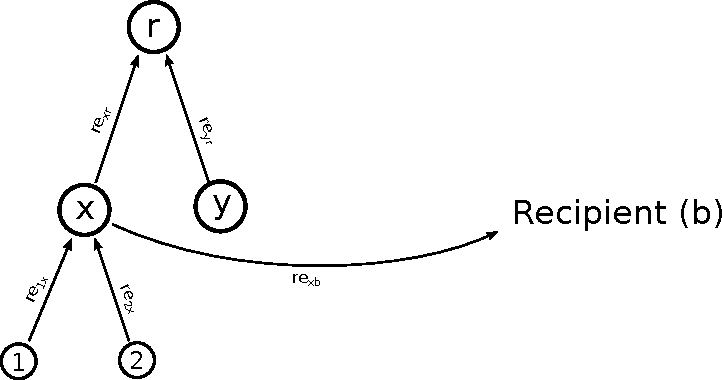
\includegraphics[width=0.45\columnwidth]{pdf/hierarchical.pdf}
    \caption{共享分层结构(如文件和文件夹)}
    \label{fig:hierarchical-pre}
\end{figure}

\subsection{批量加密数据}

        当我们拥有一个文件的对称加密密钥时,恶意接收方有可能下载所有加密的对称密钥,并在访问时解密,而无需下载过多的数据。 他可以稍后使用这些对称密钥来解密大量数据。 这被称为“密钥抓取攻击”。
    
    在出现这种问题的应用程序中,我们可以使用对数据进行全有或全无转换的方法,只有下载所有文件才能解密数据。 这种方法已经发表~\cite{aont-bulk},可以在我们的密钥管理系统中使用。

\subsection{共享加密的流}

与多个用户共享加密流对像去中心化的Netflix这样的应用程序是理想的,因为路由流量的第三方不被允许看到这些内容。

    原理很简单:数据流中的每个数据块用随机的DEK加密,EDEK使用每个频道的公钥生成。但是,与\kms 进行往返需要花费时间。 因此,将下一个数据区块的EDEK包括在前一个块中是合理的。
    
    而且,对于流媒体内容的用例来说,密钥抓取攻击尤其成问题。 因此,我们应该将电影区块视为批量数据并进行相应的加密~\cite{aont-bulk}。
    
    像往常一样,流的消费者拥有自己的密钥对,并要求矿工节点使EDEK可以被消费者解密。 矿工还可以确保消费者已支付订阅费用,如果没有则拒绝重加密。


\subsection{基于时间和基于条件的策略}

    尽管我们不信任处理加密数据或密钥的矿工,但我们仍然相信他们能够控制存储重加密密钥的时间。最简单的策略是基于时间的:只有在规定的时间间隔内才允许重加密,如果将来不需要重加密,则应该删除重加密密钥。
    
    可以创建更复杂的策略,比如重加密基于以下条件 -待完成某个交易。 这使得按内容付费的DRM和为金融交易托管而存储私密数据的应用程序成为可能。


\subsection{密钥轮换}
\label{sec:key-rotation}

    许多代理重加密算法可以应用多次,包括BBS98~\cite{BBS98}。 因此,代理重加密可以用于密钥轮换。 密钥轮换允许用旧密钥加密的所有EDEK再用新密钥加密。
    
    数据所有者需要在两个版本的密钥之间生成重加密密钥$re_{v1\rightarrow v2}$,本质上是与未来的自我共享数据。 现在,重加密节点(假设加密存储是公开的,例如IPFS)将下载EDEKs并应用转换。 对于这个操作,由于数据的“发送方”和“接收方”本质上是同一个人,所以不存在合谋风险。

\section{设计智能合约}
\label{sec:smart-contract}

为了提供重加密服务,节点需要将币发送到智能合约(同时指定锁定时间)。在时间到期之后,节点可以从中收回代币。目的是如果他们正确地提供重加密服务,就奖励挖矿节点。

    在最初的版本实现中,我们将确保节点保持在线状态并正确地重加密数据,而不需要匿名(第~\ref{sec:anonymity}节)。 我们希望节点能够变得专业化,并在其安全性方面进行大量的投入,类似于其他网络中发生的情况。 因此,我们对提供重加密服务的结点有最小持币数要求 – $s_{\min}$。 这也自然地限制了节点的数量,类似于在DASH加密货币~\cite{dash:whitepaper}中设置主节点的机制。
    
    币的数量是公开的,所以网络的客户端可以自己决定在部署重加密密钥时是否同时部署节点。 客户端(Alice)负责随机分发重加密的密钥。 我们不强制Alice在区块链上选择的随机性。
    
    我们将第$i$个活跃的(即币被锁定的)矿工称之为$d_i$。 锁定的币总额为:

\begin{equation}
    D = \sum_1^k d_i,
\end{equation}

其中$k$是矿工总数。 第$i$位矿工从一个策略获得重加密密钥的概率是:

\begin{equation}
    p_i = n\frac{d_i}{D},\qquad\text{in the limit}\quad \forall i: n p_i \ll 1,
\end{equation}

        其中$n$是我们分割重加密密钥的分段个数(第~\ref{sec:split-key}章)。

    选择随机节点来处理重加密密钥的方式如下~(\figref{fig:random-nodes}): 所有的节点都是随机排列的,并且放置在从坐标$x=0$开始长度为$D$的坐标上。因此,第$i$个节点的坐标将是:
    
\begin{figure}
    \centering
    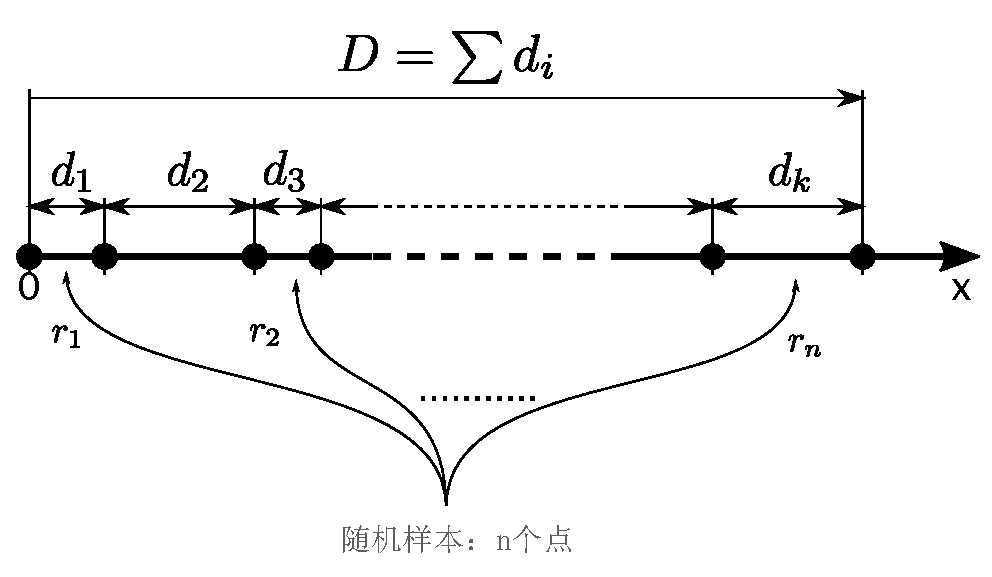
\includegraphics[width=0.6\textwidth]{pdf/miners-ruler.pdf}
    \caption{根据PoS选择随机节点。 每个节点$d_i$的权重被表示为线段。 这些线段连接在一起,形成一根长度为$D$的较大线段。随机节点由从x = 0到x = D分布的随机点中选择}
    \label{fig:random-nodes}
\end{figure}
\begin{equation}
    x_i = \sum_{j=1}^{i-1} d_j.
\end{equation}

        在部署策略时,Alice选择$n$个随机数字:
    
\begin{equation}
    \forall j=1..n: r_j \in [0, D).
\end{equation}

        在不失一般性的情况下,假设数$r_j$被选中。 那么选定的矿工$i_j$的索引就是所选坐标对应的矿工的索引:

\begin{equation}
    \forall i_j: x_{i_j} \le r_j, x_{i_j + 1} > r_j.
\end{equation}

        有些数字可能会落在对应同一矿工的线段上。在这种情况下,Alice删除重复的$i_j$ ,并以相同的方式生成更多矿工索引$i_j$ ,直到选择了所需数量的矿工($n$)。

        我们将可能的测试组合称之为是一个普遍的“ping”。这包括:
\begin{itemize}
    \item 实际的ping(网络中节点是否显示?);
    \item 检查旧的但仍活跃的重加密策略是否有效;
    \item 检查创建-重加密-撤销序列是否有效;
    \item 如果从不同地址发出请求,检查上面的重加密策略是否工作,而不是与挖掘节点相关。
\end{itemize}
        当执行这个“ping”时,可以选择只做检测可用性的必要测试。 例如,如果一个节点脱机,那么(非常轻量的)实际的ping就足以确定节点的状态。
    
    
    现在,我们要设计一个节点系统,每隔h个块进行自我检查(例如,$h=10$)。 这个想法是,节点打赌哪个节点行为不当,挖矿奖励取决于他们的猜测是否正确。“正确的”猜测被认为是多数结点投票选择的那个,这是由智能合约从所有节点的投票中计算得出。
    
    如果每$h$个块我们检查每个节点,协议将不能很好地与系统$N$中的节点总数成比例。 因此,只有一部分节点(例如$k=\sqrt{N}$)将被检查。 例如,如果有$100,000$个节点在线并且以太坊块时间是$24$秒(当前值),则大约每隔$21$个小时每个节点的健康状况将被检查一遍。 要验证的节点的选择可以由当前的验证节点交换随机的离线字节并计算这些随机字节排序和加入的哈希来完成。 不参与验证的节点将无法区分是否受到挑战或接收到真实的客户端请求。

    所有节点执行健康检查也是不可行的。 因此,一部分节点(例如,按照汉明距离离当前块哈希最近的$\sqrt{N}$个节点)将能够在当前轮次中获得健康检查的奖励。 如果发现节点不健康,则会受到惩罚,失去自上次健康检查以来获得的平均奖励。

    检查节点输出重加密的正确性是可行的。为了做到这一点,数据的拥有者可以准备一个“挑战包” - 这个数据不对应任何敏感数据,但专门用来挑战重加密节点。“挑战包”由输入密文和期望的重加密的输出组成(这种方法仅适用于没有概率输出的代理重加密算法)。数据的接收方可以解密挑战包,并证明重加密节点失败或无法正确地重加密数据。

    挑战其他重密节点的节点本质上是投票哪个节点行为不当,并对投票结果打赌。 在每个节点进行投票之前,挑战者节点应该无法先行得知其他节点的投票情况。 因此,他们首先通过展示加盐票的哈希来投票,随后证明他们有实际的投票和盐($n$个随机数)来产生这些哈希。

\section{代币经济}
\label{sec:token}

协议经济由矿工网络组成,矿工网络提供稀缺资源,并在消耗资源时得到回报。 在\kms 中,矿工是重加密节点。任何人都可以成为矿工,根据提供的重加密操作的数量来区分他们的奖励。 获得稀缺的重加密服务必须加以控制并分配给最高价值的用途。 我们实现这一目标的机制是\kms 代币(NKMS)。 NKMS既是对矿工贡献工作的奖励,也是消费者(数据所有者)为获得重加密服务而付出的费用。 最重要的是,代币也激励了计算的正确性和系统的安全性。

\subsection{代币分发}

        矿工可以持有一定数量的重加密密钥,这与他们作为抵押资产所持有的代币数量成比例,其由智能合约锁定。 矿工们既可以提供重加密服务,又可以重加密数据。矿工费既可以由数据所有者支付,也可以由数据使用者支付。在DAOs通过去中心化DRM分发内容的用例中,后者会更为重要。
    
        此外,如果矿工在线并准备好提供服务,矿工可能会获得“可用性奖励”,在智能合约(第~\ref{sec:smart-contract}节)的帮助下可以证明这一点。如果矿工离线,他们将在这段时间内丧失“可用性”补偿。
    
        如果矿工作弊并提供错误的重加密,他们将损失一部分抵押资产(第~\ref{sec:challenge-protocol}节)。
    
    我们可以阻止矿工泄漏重加密的密钥。任何人都可以使用重加密密钥的哈希来挑战矿工,如果证实重加密密钥已经泄露,矿工抵押的NKMS将被罚没。把重密密钥链接到特定的代理是可能的,以便在加密级别泄露时快速识别它们~\cite{Libert2008}。
    
    在早期当系统中用户不多时,激励重加密操作非常重要。 这就是为什么我们要引入一个奖励时间表,其中一些奖励是“挖矿”,随着时间的推移,逐渐接近零通货膨胀。 矿工$i$得到的报酬$r_i$可以表示为:
    
\begin{equation}
    r_i = \frac{d_i \cdot s}{\sum_{i=1}^k d_i} + f_i,
\end{equation}

        其中$s$是当前的回报率,$d_i$是第i个矿工的抵押资产,$f_i$是该矿工的交易总费用。 奖励率呈指数级下降,直到随时间达到平衡,最后奖励只来源于交易费:
    
\begin{equation}
    s = s_0 e^{-t/T},
\end{equation}

        其中在时间$T$之后,奖励根据影响因素$e$下降,$s_0$是初始奖励率。这个指数可以方便地在智能合约中获得,而不需要昂贵的浮点运算得出微分方程的解:
    
\begin{equation}
    s = \frac{dS}{dt}= s_0 \frac{S_{\max} - S}{S_{\max} - S(t=0)},
\end{equation}

        在$t=\infty$时$S_{\max}$是代币的最大供应量,$S(t=0)$是代币的初始供应量。时间$t$用挖矿周期而不是秒表示。

        \kms 的一个有趣属性是安全性随着网络参与者数量的增长而提高。随着越来越多的重加密节点进入网络,合谋的可能性就越小。这提高了系统的安全性和抗审查性,提供强大的网络效应和有意义的先发优势。
    
    最后,为了测试网络的安全性,我们可以设置赏金密钥 - 有一些代币的钱包私钥。任何人都可以自由地破解系统,并获得赏金。赏金被拿走就证明系统已经不安全了。同样的机制可以用来警告网络个人用户潜在的数据泄漏,通过发信号通知他们可能暴露了他们的数据私钥。


\section{用例}

        作为基本功能,\kms 为需要共享敏感数据的各种应用程序提供基础设施,具有在共识网络上以公共行为为条件进行解密操作的能力,例如发布某些消息,在特定方之间进行支付以及其他事件,可以实现一系列应用,包括:

\subsection{共享加密文件(“去中心化Dropbox”)}
\label{sec:files}

        文件可以在客户端加密,并存储在像Swarm~\cite{swarm},IPFS~\cite{whitepaper:ipfs},Sia~\cite{web:sia}或Storj ~\cite{web:storj}这样的去中心化文件系统中,或者像S3一样中心化的文件系统中。通过提供基于第三方公钥的重加密令牌,可以轻松地与授权的第三方共享文件。 通过从网络中删除重加密的令牌,可以很容易地撤销第三方的访问权限。

\subsection{端到端加密群聊(“加密Slack”)}

    代理重加密是端到端加密群组消息的理想基元,群聊需要多个参与者在频道中读取和写入消息。通过发出或撤销重加密令牌,可以轻松地在群聊中添加或删除成员。 这避免了多次加密和发送消息的开销,每人只需一次。

\subsection{患者控制的电子健康记录(EHR)}

    可以创建患者控制的EHR,患者拥有自己的数据和加密密钥,这和Epic这样的中心化系统不一样。而且,数据可以中心化存储或去中心化存储。 当病人想要与医院或保险公司分享他们的加密数据时,他们会发出一个重加密令牌,授予第三方临时访问权限。

\subsection{去中心化数字版权管理(DDRM)}
\label{sec:drm}

        加密访问控制可以用于去中心化DRM。访问控制可以嵌入到加密本身中,以便随时随地追踪数据动向。有条件的重加密令牌可以通过智能合约来控制,以便在付款后才能被释放。现在可以使用\kms~来构建去中心化Netflix服务或销售软件、应用程序、照片和其他数字内容的加密市场。

\subsection{盲身份管理}

    使用\kms~可以构建一个盲身份管理服务。ID可以在客户端进行加密,并与身份管理提供商一起存储。用户可以为被认可的应用程序创建重加密密钥。该服务为所述第三方应用程序重加密身份凭证,而身份提供者不具有访问权限。

\subsection{脚本和后端应用程序的秘密凭证管理}

        \kms~是存储任何秘密的理想选择,例如敏感的环境变量、数据库凭证和API密钥。对于脚本而言,可以在脚本的生存时间内生成重加密令牌,然后撤销。例如,开发人员可以在GitHub上安全地存储加密的数据库凭证,并在部署实例后临时授予其访问这些凭证的许可。即使GitHub存储库是公开的,证书也不能被未经授权的人使用。

\subsection{共享凭证和企业密码管理}
        \kms~可以管理员工用来访问Web服务的共享凭证。可以建立审计日志来监控谁访问了什么秘密。员工离职时,很容易撤销访问甚至回滚密钥。

\subsection{强制访问日志}

        在某些公司和企业设置中,客户端必须发布敏感文件的访问日志。这要求记录每个文件的访问权限,并且可以使用条件重加密来强制执行这些记录规则。

\subsection{移动设备管理(MDM)和撤销}
\label{sec:mdm}

    在企业MDM设置中,可为有效设备创建重加密令牌。当设备丢失或报废或员工离职时,可以删除重加密令牌以撤销对设备的访问权限。这避免了重新组织分级密钥树的问题。

\subsection{\kms~的私有使用}

        为了使传统企业(金融、医疗、政府或物联网公司)受益,\kms~可以被私有部署。 它可以部署成私有或联盟的区块链,从而联盟化(矿工由企业联盟控制的预先选定的节点替代)甚至中心化(一个组织控制所有重加密密钥)。这些使用仍然可以享受代理重加密的安全优势,但是抗审查能力不会那样有效。

\section{概要}
        
    \kms~是去中心化密钥管理服务和密码访问控制层,用于区块链和去中心化应用程序。开发人员和企业都可以利用它来创建高度安全的应用程序,可应用于医疗医疗保健、金融服务等。通过将私人数据共享和计算带入公有链,\kms~使从加密内容市场到秘密凭证管理再到病人控制的电子健康记录成为可能。


\section{致谢}

        我们要感谢来着斯蒂文斯理工学院的Giuseppe Ateniese和马拉加大学的Isaac Agudo Ruiz对代理重加密算法的帮助。我们也感谢弗吉尼亚大学的戴夫·埃文斯(Dave Evans)为我们公司在整个生命周期中提供咨询服务,并感谢他在多方计算方面的最新进展。 还有Stefano Bernardi,Tom Ding和其他许多人在代币经济学的帮助。
    

\bibliography{kms-whitepaper}

\end{document}
